\documentclass[10pt,a4paper]{article}
\input{AEDmacros}
\usepackage{etoolbox}
\usepackage{adjustbox}
\usepackage{inconsolata}
\usepackage{tcolorbox}
\usepackage{xcolor}
\usepackage{ragged2e}
\usepackage{changepage}
\usepackage{amssymb}
\usepackage[outputdir=out]{minted}
\DeclareRobustCommand{\ttfamily}{\fontencoding{T1}\fontfamily{lmtt}\selectfont}

\lstset{
  basicstyle=\ttfamily,
  numbers=none,
  frame=none,
  xleftmargin=10px,
  aboveskip=0pt
}
\newcommand{\vacio}{\emptyset}
\newcommand{\limn}{\lim_{n \to \infty}}
\newcommand{\ceil}[1]{%
  \left\lceil #1 \right\rceil%
}
\newcommand{\reales}{\mathbb{R}}
\newcommand{\limite}[2]{%
  \lim_{#1 \to #2}
}

\newenvironment{groupIzq}[1]{%
  \begin{list}{}{%
      \setlength{\leftmargin}{#1}%
      \setlength{\topsep}{0pt} % Elimina el espacio superior
      \setlength{\partopsep}{0pt} % Asegura que no haya espacio extra
    }
  \item[]
}{%
  \end{list}
}
\newcommand{\demoline}{\vspace{0.5em}}

\newcommand{\Indent}{\hspace*{0.75cm}}
\newcommand{\MiniIndent}{\hspace*{0.325cm}}
\newcommand{\Int}{\ensuremath{int}}

\newcommand{\Extends}[2]{%
  \noindent\ensuremath{\texttt{\textbf{#1}}\ \texttt{\textbf{extends}}\ #2}%
  \par
}
\newcommand{\Array}[1]{\ensuremath{Array \texttt{<}#1\texttt{>}}}
\newcommand{\Tupla}[1]{\ensuremath{Tupla \texttt{<}#1\texttt{>}}}
\newcommand{\Tuple}[1]{\ensuremath{Tuple \texttt{<}#1\texttt{>}}}
\newcommand{\Clase}[2]{\texttt{#1<#2>}}
\newcommand{\Type}[2]{%
  \noindent\ensuremath{\texttt{\textbf{#1}} = #2}%
  \par
}
\newcommand{\primitiva}[1]{\ensuremath{#1}}
\newcommand{\Arr}[1]{\ensuremath{Array \langle #1 \rangle}}
\newcommand{\conj}[1]{\ensuremath{conj \langle #1 \rangle}}
\newcommand{\union}{\cup}
\newcommand{\interseccion}{\cap}
\newcommand{\Struct}[1]{\ensuremath{\texttt{Struct} \langle \texttt{#1} \rangle}}
\newcommand{\StructField}[2]{\normalfont\ttfamily{#1}: \ensuremath{#2}}
\newcommand{\Title}[1]{%
  \raggedright
  \noindent{\textbf{#1}}%
  \justifying
  \vspace{1em}%
}

\newcommand{\TitlePar}[1]{%
  \raggedright
  \noindent{\textbf{#1}}%
  \justifying%
}

\newcommand{\Var}[2]{%
  \noindent\texttt{var \textbf{#1}}: #2 \par
}
\newenvironment{Vars}{%
  \begin{flushleft} % Alineación a la izquierda
}{%
  \end{flushleft}
  \vspace{1em} % Salto de línea final
}

\newenvironment{ModuloImplements}[2]{%
  \raggedright
  \texttt{Modulo #1\ implements\ #2\ \{}
  \justifying
  \begin{adjustwidth}{2em}{0em}
}{%
  \end{adjustwidth}
  \texttt{\}}%
}

\definecolor{lightgray}{gray}{1}
\definecolor{darkgray}{gray}{0.65}
\newcommand{\comentario}[1]{%
  \noindent{\normalfont\bfseries\ttfamily\small\textcolor{darkgray}{\% #1\ \ \%} \par}%
}

\newtcolorbox{ImplementationCodeBoxFixedWithParam}[1]{colback=lightgray!20, colframe=white, boxrule=0pt, left=5pt, right=5pt, top=5pt, bottom=5pt, width=#1}
\newtcolorbox{ImplementationCodeBoxFixed}{colback=lightgray!20, colframe=white, boxrule=0pt, left=5pt, right=5pt, top=5pt, bottom=5pt, width=0.8\linewidth}
\newtcolorbox{ImplementationCodeBox}{colback=lightgray!20, colframe=white, boxrule=0pt, left=5pt, right=5pt, top=5pt, bottom=5pt, width=\dimexpr\textwidth-2em\relax}
\definecolor{lightgray}{RGB}{220,220,220}
\newenvironment{ImplementationCode}[1]{%
  \VerbatimEnvironment
  \vspace{-0.2em}
  \begin{ImplementationCodeBoxFixedWithParam}{#1}
  \flushleft
  \begin{adjustbox}{minipage=\dimexpr\textwidth-2em\relax, margin=0pt}
  \begin{minted}[linenos, xleftmargin=-2.4em, numbersep=-2.5em]{java}%
}{
  \end{minted}
  \end{adjustbox}
  \vspace{-0.25em}
  \end{ImplementationCodeBoxFixedWithParam}
  \fussy
}

\usepackage{graphicx}
\usepackage{geometry}

\geometry{paperwidth=21cm, paperheight=80cm}

\begin{document}

\Title{Ejercicio 1}

\begin{figure}[h]
  \centering
  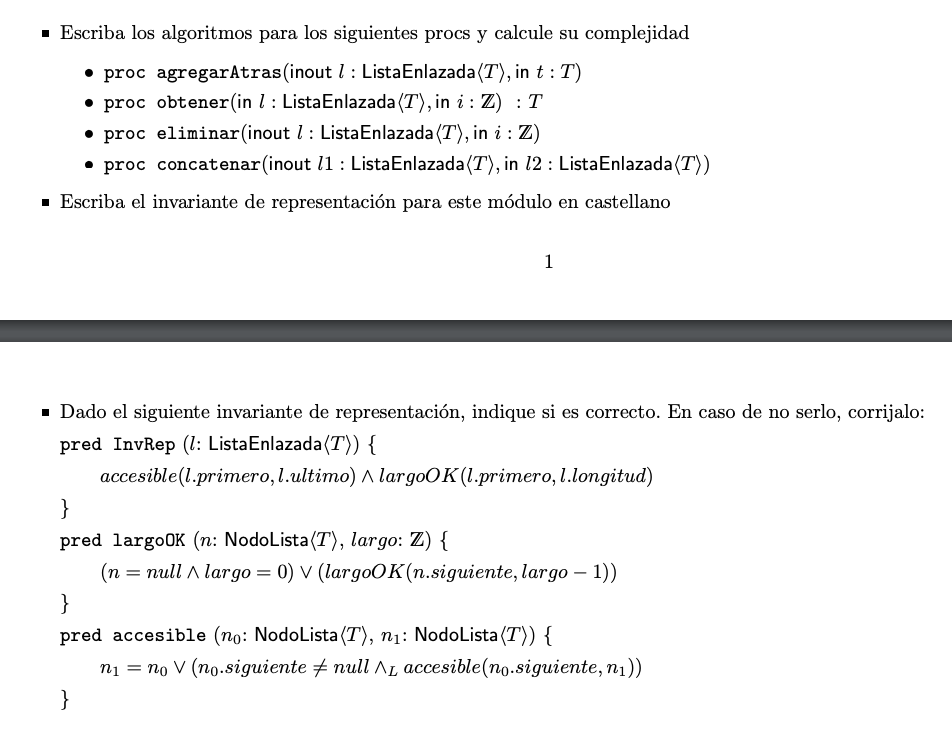
\includegraphics[width=\textwidth]{images/nuevo_ejercicio_1.png}
  \caption{Enunciado Problema 1}
  \label{fig:ej_1}
\end{figure}

\Type{NodoLista<T>}{\Struct{\StructField{valor}{T}, \StructField{siguiente}{\Clase{NodoLista}{T}}}}
\vspace{1em}
\begin{ModuloImplements}{ListaEnlazada<T>}{Secuencia<T>}
  \begin{Vars}
    \Var{primero}{\Clase{NodoLista}{T}}
    \Var{ultimo}{\Clase{NodoLista}{T}}
    \Var{longitud}{\primitiva{int}}
  \end{Vars}

  \pred{listaDe}{nodo: \Clase{NodoLista}{T}, s: \TLista{T}}{
    (|s| = 0 \implica nodo = Null) \land \\
    (|s| > 0 \implica (nodo \neq Null \yLuego nodo.valor = head(s) \yLuego listDe(nodo.siguiente, tail(s))))
  }

  \pred{abs}{l: \Clase{ListaEnlazada}{T}, l': \Clase{Seceuencia}{T}}{
    |l'.s| = l.longitud \yLuego listaDe(l.primero, l'.s)
  }
  \pred{invRep}{l: \Clase{ListaEnlazada}{T}}{
    l.longitud \geq 0 \land 
    \\ (l.longitud = 0 \implica (l.primero = Null \land l.ultimo = Null)) \land
    \\ (l.longitud = 1 \implica (l.primero \neq null \land l.primero = l.ultimo)) \land
    \\ (l.longitud > 1 \implica (l.primero \neq Null \land l.ultimo \neq Null \land l.primero \neq l.ultimo)) \yLuego 
    \\ sinCiclos(l.primero, \{\}) \yLuego largoOK(l.primero, l.longitud) \land alcanzable(l.primero, l.ultimo)
  }
  \pred{sinCiclos}{nodo: \Clase{NodoLista}{T}, visitados: \conj{\Clase{NodoLista}{T}}}{
    nodo = Null \oLuego (nodo \notin visitados \yLuego sinCiclos(nodo.siguiente, visitados \union \{nodo\}))
  }
  \pred{largoOK}{nodo: \Clase{NodoLista}{T}, longitud: \ent}{
    (longitud = 0 \implica nodo = null) \land \\
    (longitud \ne 0 \implica nodo \neq null \yLuego largoOK(nodo.siguiente, longitud - 1))
  }
  \pred{alcanzable}{$n_0$: \Clase{NodoLista}{T}, $n_1$: \Clase{NodoLista}{T}}{
    (n_0 = n_1) \lor (n_0 \neq Null \yLuego alcanzable(n_0.siguiente, n_1))
  }
  \vspace{1em}
  \begin{proc}{agregarAtras}{\Inout l: \Clase{ListaEnlazada}{T}, \In t: T}{}
    \begin{ImplementationCode}{320px}
      var nodo: NodoLista<T>
          nodo:= new NodoLista<T>()
          nodo.valor:= t
          nodo.siguiente:= null
      
      if l.primero == null && l.ultimo == null
        l.primero:= nodo
      else
        l.ultimo.siguiente:= nodo
      endif

      l.ultimo:= nodo
      l.longitud:= l.longitud + 1

      return
    \end{ImplementationCode}
  \end{proc}
  \begin{proc}{obtener}{\In l: \Clase{ListaEnlazada}{T}, \In i: int}{T}
    \begin{ImplementationCode}{320px}
      var nodoActual: NodoLista<T>
          nodoActual:= l.primero

      while (nodoActual != null && i > 0) do
        nodoActual:= nodoActual.siguiente
        i:= i - 1
      endwhile

      return nodoActual.valor
    \end{ImplementationCode}
  \end{proc}
  \begin{proc}{eliminar}{\Inout l: \Clase{ListaEnlazada}{T}, \In i: int}{}
    \begin{ImplementationCode}{360px}
      if i == 0 then
        l.primero:= l.primero.siguiente
        l.ultimo:= l.longitud > 1 ? l.ultimo : null 
      else
        var nodoActual: NodoLista<T>
            nodoActual:= l.primero

        while (i > 1) do
          nodoActual:= nodoActual.siguiente
          i:= i - 1
        endwhile

        nodoActual.siguiente:= nodoActual.siguiente.siguiente
        l.ultimo:= nodoActual.siguiente != null ? l.ultimo : nodoActual 
      endif

      l.longitud:= l.longitud - 1

      return
    \end{ImplementationCode}
  \end{proc}
  \begin{proc}{concatenar}{\Inout lista1: \Clase{ListaEnlazada}{T}, \In lista2: \Clase{ListaEnlazada}{T}}{}
    \begin{ImplementationCode}{350px}
      var nodoActual: NodoLista<T>
          nodoActual:= lista2.primero

      while (nodoActual != null) do
        agregarAtras(lista1, nodoActual.valor)
        nodoActual:= nodoActual.siguiente
      endwhile

      return
    \end{ImplementationCode}
  \end{proc}
\end{ModuloImplements}

\newpage

\begin{figure}[h]
  \centering
  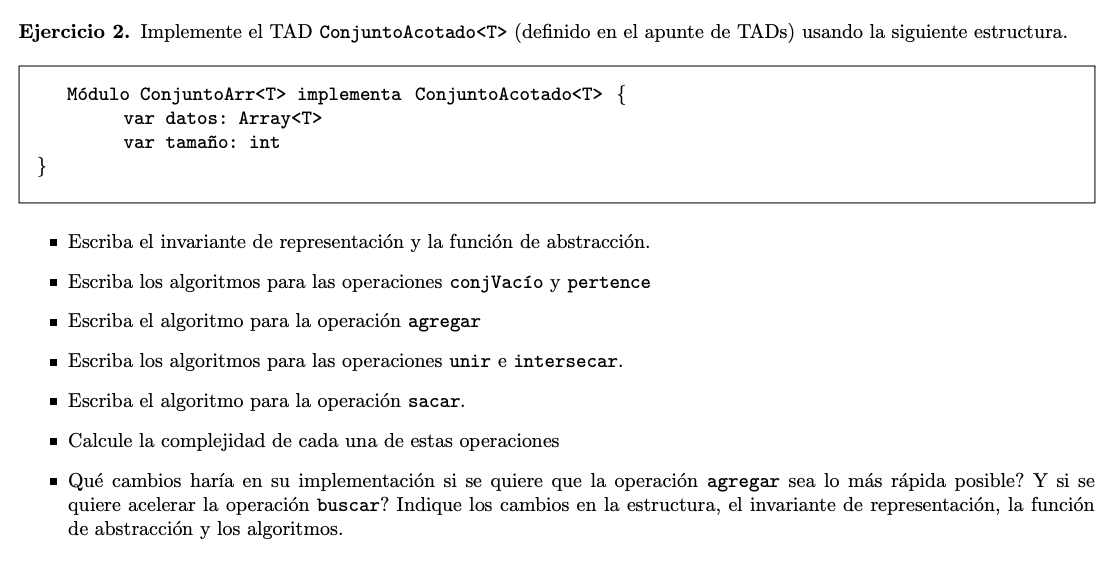
\includegraphics[width=\textwidth]{images/nuevo_ejercicio_2.png}
  \caption{Enunciado Problema 2}
  \label{fig:ej_2}
\end{figure}
\vspace{1em}
\begin{ModuloImplements}{ConjuntoAcotadoArr<T>}{ConjuntoAcotado<T>}
  \begin{Vars}
    \Var{datos}{\Array{T}}
    \Var{tamaño}{\primitiva{int}}
  \end{Vars}

  \pred{sinRepetidos}{c: \Clase{ConjuntoAcotadoArr}{T}, }{
    \paraTodo[unalinea]{i, j}{\ent}{0 \leq i,j < c.tama$ñ$o \land i \neq j \implicaLuego c.datos[j] \neq c.datos[i]}
  }
  \pred{abs}{c: \Clase{ConjuntoAcotadoArr}{T}, c': \Clase{ConjuntoAcotado}{T}}{
    c'.cota=length(c.datos) \land |c'.elems|=c.tama$ñ$o \land 
    \paraTodo[unalinea]{t}{T}{t \in c'.elems \leftrightarrow t \in subseq(c.datos, 0, c.tama$ñ$o)}
  }
  \pred{invRep}{c: \Clase{ConjuntoAcotadoArr}{T}}{
    0 \leq c.tama$ñ$o \leq length(c.datos) \land
    sinRepetidos(c) \land
    \paraTodo[unalinea]{j}{\ent}{0 \leq j < c.tama$ñ$o \implicaLuego def(c.datos[j])}
  }
  \vspace{1em}
  \begin{proc}{conjVacío}{\In cota: int}{\Clase{ConjuntoAcotadoArr}{T}}
    \begin{ImplementationCode}{320px}
      var datos: Array<T>
          datos:= new Array<T>(cota)
      
      res.datos:= datos
      res.tamaño:= 0

      return res
    \end{ImplementationCode}
  \end{proc}
  \begin{proc}{pertenece}{\In c: \Clase{ConjuntoAcotadoArr}{T}, \In t: T}{Boolean}
    \begin{ImplementationCode}{320px}
      var i: int
          i:= 0
      
      while (i < c.tamaño) do
        if c.datos[i] == t then
          return true
        endif

        i:= i + 1
      endwhile

      return false
    \end{ImplementationCode}
  \end{proc}
  \comentario{agregarSiNoPertenece: For the sake of declaratividad}
  \begin{proc}{agregarSiNoPertenece}{\Inout c: \Clase{ConjuntoAcotadoArr}{T}, \In t: T}{}
    \begin{ImplementationCode}{320px}
      if !pertenece(c, t) then
        c.datos[c.tamaño]:= t
        c.tamaño:= c.tamaño + 1
      endif
      
      return
    \end{ImplementationCode}
  \end{proc}
  \begin{proc}{agregar}{\Inout c: \Clase{ConjuntoAcotadoArr}{T}, \In t: T}{}
    \begin{ImplementationCode}{320px}
      agregarSiNoPertenece(c, t)
      
      return
    \end{ImplementationCode}
  \end{proc}
  \begin{proc}{sacarPorIndice}{\Inout c: \Clase{ConjuntoAcotadoArr}{T}, \In i: int}{}
    \begin{ImplementationCode}{320px}
      c.datos[i]:= c.datos[c.tamaño - 1]
      c.tamaño:= c.tamaño - 1

      return
    \end{ImplementationCode}
  \end{proc}
  \begin{proc}{sacar}{\Inout c: \Clase{ConjuntoAcotadoArr}{T}, \In t: T}{}
    \begin{ImplementationCode}{320px}
      var i: int
          i:= 0

      while (i < c.tamaño) do
        if c.datos[i] == t then
          sacarPorIndice(c, i)

          return
        endif

        i:= i + 1
      endwhile

      return
    \end{ImplementationCode}
  \end{proc}
  \begin{proc}{unir}{\Inout c1: \Clase{ConjuntoAcotadoArr}{T}, \In c2: \Clase{ConjuntoAcotadoArr}{T}}{}
    \begin{ImplementationCode}{320px}
      var i: int
          i:= 0

      while (i < c2.tamaño) do
        agregarSiNoPertenece(c1, c2.datos[i])
        i:= i + 1
      endwhile

      return
    \end{ImplementationCode}
  \end{proc}
  \begin{proc}{intersecar}{\Inout c1: \Clase{ConjuntoAcotadoArr}{T}, \In c2: \Clase{ConjuntoAcotadoArr}{T}}{}
    \begin{ImplementationCode}{360px}
      var i: int
          i:= 0

      while (i < c1.tamaño) do              // O(n)
        if !pertenece(c2, c1.datos[i]) then // O(m)
          sacarPorIndice(c1, i)             // O(1)
        endif

        i:= i + 1
      endwhile

      return
    \end{ImplementationCode}
  \end{proc}
\end{ModuloImplements}

\newpage

\begin{figure}[h]
  \centering
  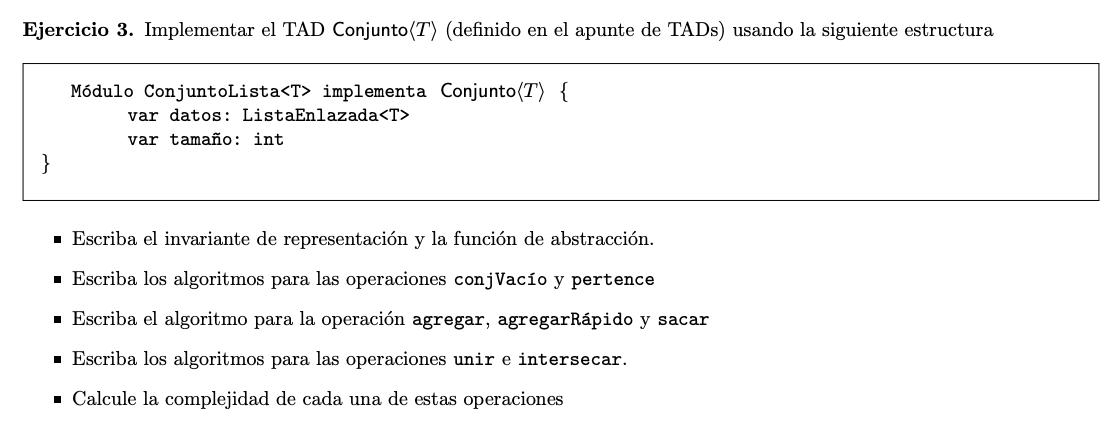
\includegraphics[width=\textwidth]{images/nuevo_ejercicio_3.png}
  \caption{Enunciado Problema 3}
  \label{fig:ej_3}
\end{figure}
\vspace{1em}
\begin{ModuloImplements}{ConjuntoLista<T>}{Conjunto<T>}
  \begin{Vars}
    \Var{datos}{\Clase{ListaEnlazada}{T}}
    \Var{tamaño}{\primitiva{int}}
  \end{Vars}
 
  \pred{sinRepetidos}{c: \Clase{ConjuntoLista}{T}} {
    \paraTodo[unalinea]{i, j}{\ent}{(0 \leq i, j < |c.datos.s| \yLuego c.datos.s[i] = c.datos.s[j]) \implica i = j}
  }
  \pred{abs}{c: \Clase{ConjuntoLista}{T}, c': \Clase{Conjunto}{T}}{
    |c'.elems| = c.tama$ñ$o \land \paraTodo[unalinea]{t}{T}{t \in c'.elems \leftrightarrow t \in c.datos.s}
  }
  \pred{invRep}{c: \Clase{ConjuntoLista}{T}}{
    c.tama$ñ$o = |c.datos.s| \land sinRepetidos(c)
  }

  \vspace{1em}
  \begin{proc}{conjVacio}{}{\Clase{ConjuntoLista}{T}}
    \begin{ImplementationCode}{360px}
      var nuevaListaEnlazada: ListaEnlazada<T>
          nuevaListaEnlazada:= new listaEnlazadaVacia()

      res.datos:= nuevaListaEnlazada
      res.tamaño:= 0

      return res
    \end{ImplementationCode}
  \end{proc}
  \begin{proc}{buscarIndicePorValor}{\In c: \Clase{ConjuntoLista}{T}, \In t: T}{Boolean}
    \begin{ImplementationCode}{360px}
      // Devuelve -1 si el elemento no pertenece
      // Devuelve 0 <= i < c.tamaño si el elemento pertenece
      var i: int
          i:= 0
      var indice: int
          indice:= -1
      
      while (i < c.datos.tamaño() && indice == -1) do
        if c.datos.obtener(i) == t then
          indice:= i
        endif
  
        i:= i + 1
      endwhile
  
      return indice
    \end{ImplementationCode}
  \end{proc}

  \begin{proc}{pertenece}{\In c: \Clase{ConjuntoLista}{T}, \In t: T}{Boolean}
    \begin{ImplementationCode}{360px}
      var indice: int
          indice:= buscarIndicePorValor(c, t)

      return indice != -1
    \end{ImplementationCode}
  \end{proc}
  \begin{proc}{agregarRapido}{\Inout c: \Clase{ConjuntoLista}{T}, \In t: T}{}
    \begin{ImplementationCode}{360px}
      c.datos.agregarAtras(t)
      c.tamaño = c.datos.tamaño()

      return
    \end{ImplementationCode}
  \end{proc}
  \comentario{agregarSiNoPertenece: For the sake of declaratividad}
  \begin{proc}{agregarSiNoPertenece}{\Inout c: \Clase{ConjuntoLista}{T}, \In t: T}{}
    \begin{ImplementationCode}{360px}
      if !pertenece(c, t) then
        agregarRapido(c, t)
      endif

      return
    \end{ImplementationCode}
  \end{proc}
  \begin{proc}{agregar}{\Inout c: \Clase{ConjuntoLista}{T}, \In t: T}{}
    \begin{ImplementationCode}{360px}
      agregarSiNoPertenece(c, t)

      return
    \end{ImplementationCode}
  \end{proc}
  \begin{proc}{sacar}{\Inout c: \Clase{ConjuntoLista}{T}, \In t: T}{}
    \begin{ImplementationCode}{360px}
      if pertenece(c, t) then
        var indice: int
            indice:= buscarIndicePorValor(c, t)

        c.datos.eliminar(indice)
        c.tamaño = c.datos.tamaño()
      endif

      return
    \end{ImplementationCode}
  \end{proc}
  \begin{proc}{unir}{\Inout c1: \Clase{ConjuntoLista}{T}, \Inout c2: \Clase{ConjuntoLista}{T}}{}
    \begin{ImplementationCode}{360px}
      var i: int
          i:= 0
      
      while (i < c2.tamaño()) do
        agregarSiNoPertenece(c1, c2.datos.obtener(i))
        i:= i + 1
      endwhile
    \end{ImplementationCode}
  \end{proc}
  \begin{proc}{intersecar}{\Inout c1: \Clase{ConjuntoLista}{T}, \In c2: \Clase{ConjuntoLista}{T}}{}
    % vamos a usar !pertenece y en ese caso borramos de c1.
    \begin{ImplementationCode}{360px}
      var nuevaListaEnlazada: ListaEnlazada<T>
          nuevaListaEnlazada:= new listaEnlazadaVacia()

      var i: int
          i:= 0
      
      while (i < c1.tamaño()) do
        if pertenece(c2, c1.datos.obtener(i)) then
          nuevaListaEnlazada.agregarAtras(c1.datos.obtener(i))
        endif
        i:= i + 1
      endwhile

      c.datos = nuevaListaEnlazada
      c.tamaño = c.datos.tamaño()
    \end{ImplementationCode}
  \end{proc}
\end{ModuloImplements}

\newpage
\Title{Ejercicio 4}

\begin{figure}[h]
  \centering
  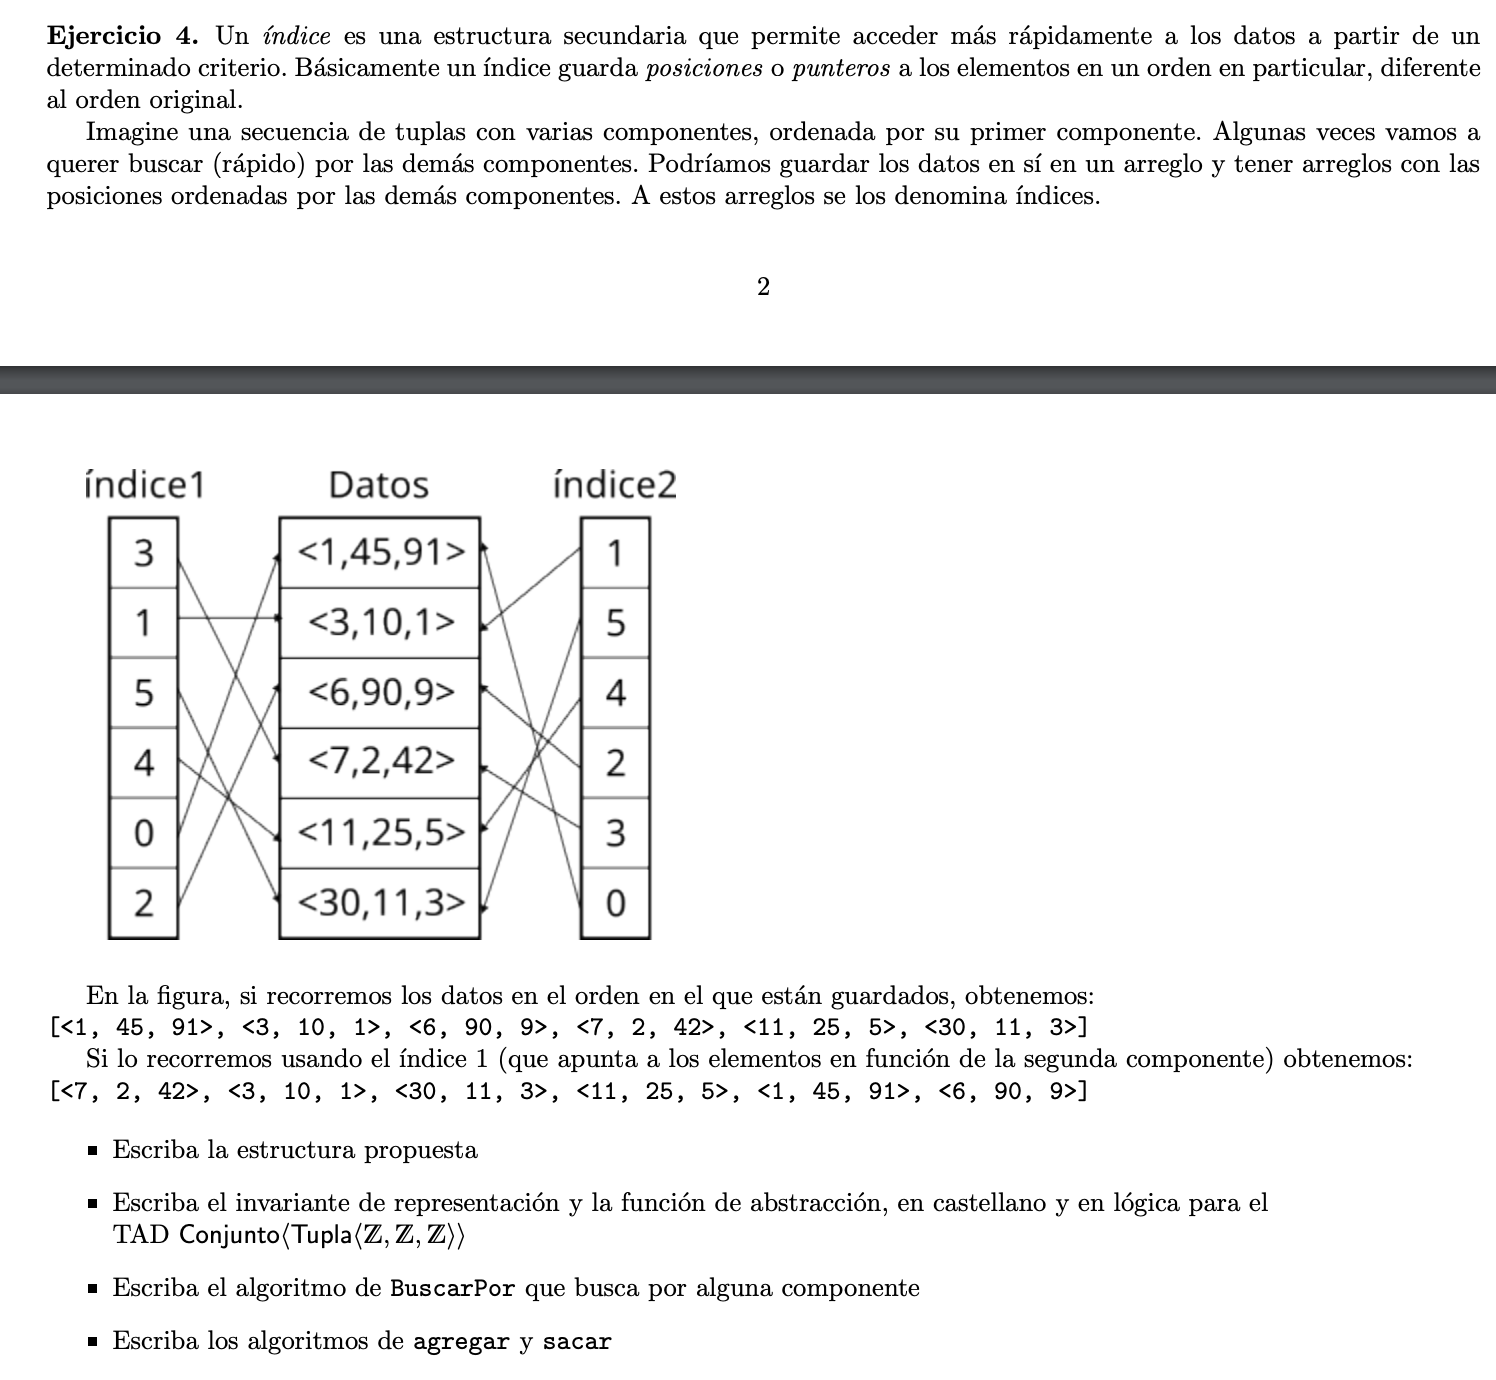
\includegraphics[width=\textwidth]{images/nuevo_ejercicio_4.png}
  \caption{Enunciado Problema 4}
  \label{fig:ej_4}
\end{figure}


\Type{Tupla}{\Tuple{int, int, int}}
\vspace{0.5em}
\begin{ModuloImplements}{ConjuntoRapido}{{\Clase{Conjunto}{\Tupla{\ent, \ent, \ent}}}}
  \begin{Vars}
    \Var{elems}{\Array{Tupla}}
    \Var{ordenadosPorCoord0}{\Array{int}}
    \Var{ordenadosPorCoord1}{\Array{int}}
    \Var{ordenadosPorCoord2}{\Array{int}}
  \end{Vars}

  \pred{indicesValidos}{c: \texttt{ConjuntoRapido}}{
    \paraTodo[unalinea]{j}{\ent}{j \in ordenadosPorCoord0 \leftrightarrow 0 \leq j < length(c.elems)} \land \\
    \paraTodo[unalinea]{j}{\ent}{j \in ordenadosPorCoord1 \leftrightarrow 0 \leq j < length(c.elems)} \land \\
    \paraTodo[unalinea]{j}{\ent}{j \in ordenadosPorCoord2 \leftrightarrow 0 \leq j < length(c.elems)}
  }
  \pred{sinRepetidosPorCoordenada}{c: \texttt{ConjuntoRapido}}{
    \paraTodo[unalinea]{coord}{\ent}{0 \leq coord \leq 2 \implicaLuego (
      \\\Indent \paraTodo[unalinea]{i, j}{\ent}{(0 \leq i, j < length(c.elems) \yLuego c.elems[i][coord] = c.elems[j][coord]) \implica i = j}
    \\)}
  }
  \pred{indicesOrdenados}{s: \Array{int}, coord: int}{
    0 \leq coord \leq 2 \yLuego \\
    \paraTodo[unalinea]{j}{\ent}{0 \leq j < (length(s) - 1) \implicaLuego (
      \\\Indent c.elems[s[j]][coord] < c.elems[s[j + 1]][coord]
    \\)}
  }
  \pred{ordenados}{c: \texttt{ConjuntoRapido}}{
    indicesOrdenados(ordenadosPorCoord0, 0) \land \\
    indicesOrdenados(ordenadosPorCoord1, 1) \land \\
    indicesOrdenados(ordenadosPorCoord2, 2)
  }
  \vspace{1em}
  \comentario{Los tipos viven en $"$mundos$"$ distintos, pero no estoy seguro como hacerlo...}
  \pred{abs}{c: \texttt{ConjuntoRapido}, c': \Clase{Conjunto}{\Tupla{\ent, \ent\, \ent}}}{
    |c'.elems|=length(c.elems) \land \\
    \paraTodo[unalinea]{t}{\Tupla{\ent, \ent, \ent}}{t \in c'.elems \leftrightarrow t \in c.elems}
  }
  \pred{invRep}{c: ConjuntoRapido}{
    length(c.elems)=length(ordenadosPorCoord1)=length(ordenadosPorCoord2) \yLuego \\
    indicesValidos(c) \yLuego sinRepetidosPorCoordenada(c) \land ordenados(c)
  }
  \vspace{1em}
  \begin{proc}{obtenerOrdenadosPorCoord}{\In c: \texttt{ConjuntoRapido}, coord: int}{\Array{int}}
    \begin{ImplementationCode}{360px}
      if coord == 0 then
        return c.ordenadosPorCoord0
      endif

      if coord == 1 then
        return c.ordenadosPorCoord1
      endif

      return c.ordenadosPorCoord2
    \end{ImplementationCode}
  \end{proc}
  \begin{proc}{actualizarOrdenadosPorCoord}{
    \\\Indent \Inout c: \texttt{ConjuntoRapido},
    \\\Indent coord: int,
    \\\Indent ordenadosPorCoord: \Array{int}
  \\}{}
    \begin{ImplementationCode}{360px}
      if coord == 0 then
        c.ordenadosPorCoord0:= ordenadosPorCoord
        return
      endif

      if coord == 1 then
        c.ordenadosPorCoord1:= ordenadosPorCoord
        return
      endif

      c.ordenadosPorCoord2:= ordenadosPorCoord
      return
    \end{ImplementationCode}
  \end{proc}
  \begin{proc}{buscarPorCoord}{\In c: \texttt{ConjuntoRapido}, \In coord: int, \In valorCoord: int}{Tupla}
    \begin{ImplementationCode}{420px}
      var largo: int
          ordenadosPorCoord: Array<int>
          largo:= length(ordenadosPorCoord)
          ordenadosPorCoord:= obtenerOrdenadosPorCoord(c, coord)

      var low: int
      var high: int
          low:= 0
          high:= largo - 1
  
      while (low <= high && low < largo) do
          mid:= floor((low + high) / 2)
          pivot:= c.elems[ordenadosPorCoord[mid]][coord]
  
          if pivot < valorCoord then
              low:= mid + 1
          else
              high:= mid - 1
          endif
      endwhile
  
      return c.elems[ordenadosPorCoord[low]][coord]
    \end{ImplementationCode}
  \end{proc}
  \newpage
  \begin{proc}{agregarEnOrdenadosPorCoord}{\Inout c: \texttt{ConjuntoRapido}, \In coord: int, \In valorCoord: int}{}
    \begin{ImplementationCode}{460px}
      var ordenadosPorCoord: Array<int>
          ordenadosPorCoord:= obtenerOrdenadosPorCoord(c, coord)

      // En este caso, elems tiene exactamente un elemento, y agrego su índice: 0.
      if length(ordenadosPorCoord) == 0:
        actualizarOrdenadosPorCoord(c, coord, new Array<int>(1)[0])
        return
      endif

      var nuevoOrdenadosPorCoord: Array<int>
          nuevoOrdenadosPorCoord:= new Array<int>(length(ordenadosPorCoord) + 1)

      // Si bien acá se podría hacer un búsqueda binaria para obtener
      // el índice para la nueva posición, eso no reducirá la complejidad del algoritmo
      var posicionValorCoord: int
          posicionValorCoord:= 0
      
      while (c.elems[ordenadosPorCoord[posicionValorCoord]][coord] < valorCoord) do
        posicionValorCoord:= posicionValorCoord + 1
      endwhile

      // Copio la porción del arreglo que mantiene el orden inferior a posicionValorCoord
      var i: int
          i:= 0

      while (i < posicionValorCoord) do
        nuevosOrdenadosPorCoords[i]:= ordenadosPorCoord[i]
        i:= i + 1
      endwhile

      // Inserto el índice correspondiente al último elemento de c.elems
      nuevosOrdenadosPorCoords[posicionValorCoord]:= length(c.elems) - 1

      // Copio la porción del arreglo que mantiene el orden superior a posicionValorCoord
      i:= posicionValorCoord + 1

      while (j <= length(ordenadosPorCoord)) do
        nuevosOrdenadosPorCoords[i]:= ordenadosPorCoord[i - 1]
        i:= i + 1
      endwhile
      
      // Actualizo el arreglo correspondiente para esta coord
      actualizarOrdenadosPorCoord(c, coord, nuevosOrdenadosPorCoords)

      return
    \end{ImplementationCode}
  \end{proc}
  \begin{proc}{agregar}{\Inout c: \texttt{ConjuntoRapido}, \In t: Tupla}{}
    \begin{ImplementationCode}{360px}
      var nuevosElems: Array<Tupla>
          nuevosElems:= new Array<Tupla>(length(c.elems) + 1)
      
      var i: int
          i:= 0

      while (i < length(c.elems)) do
        nuevosElems[i]:= c.elems[i]
        i:= i + 1
      endwhile

      nuevosElems[i]:= t

      c.elems:= nuevosElems
      agregarEnOrdenadosPorCoord(c, 0, t[0])
      agregarEnOrdenadosPorCoord(c, 1, t[1])
      agregarEnOrdenadosPorCoord(c, 2, t[2])

      return
    \end{ImplementationCode}
  \end{proc}
  \begin{proc}{sacar}{\Inout c: \texttt{ConjuntoRapido}, \In t: Tupla}{T}
    \begin{ImplementationCode}{360px}
      // @todo
    \end{ImplementationCode}
  \end{proc}
\end{ModuloImplements}

\newpage
\Title{Ejercicio 5}

\begin{figure}[h]
  \centering
  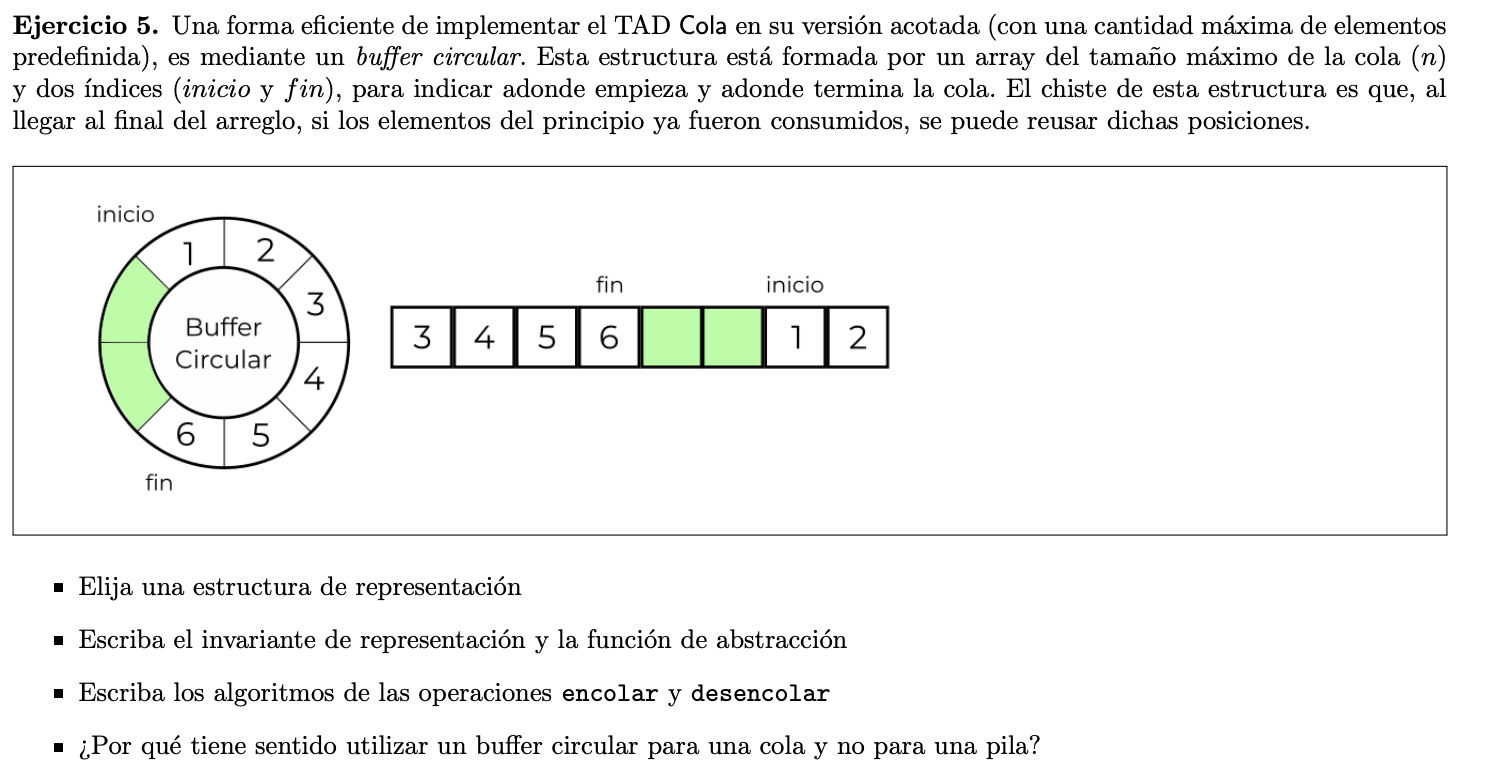
\includegraphics[width=\textwidth]{images/nuevo_ejercicio_5.png}
  \caption{Enunciado Problema 5}
  \label{fig:ej_5}
\end{figure}

\begin{ModuloImplements}{\Clase{ColaCirciular}{T}}{\Clase{ColaAcotada}{T}}
  \begin{Vars}
    \Var{elems}{\Array{T}}
    \Var{inicio}{int}
    \Var{fin}{int}
  \end{Vars}

  \aux{cantidadElementosDeInicioAFin}{c: \Clase{ColaCircular}{T}}{\ent}{
    c.fin - c.inicio
  }
  \aux{cantidadElementosDeFinAInicio}{c: \Clase{ColaCircular}{T}}{\ent}{
    (length(c.elems) - inicio) + (c.fin)
  }
  \aux{cantidadElementos}{c: \Clase{ColaCircular}{T}}{\ent}{
    \\\Indent \IfThenElse{c.inicio < c.fin}{cantidadElementosDeInicioAFin(p)}{cantidadElementosDeFinAInicio(p)}
  }
  \vspace{1em}
  \pred{abs}{c: \Clase{ColaCircular}{T}, c': \Clase{ColaAcotada}{T}}{
    c'.cota=length(c.elems) \land |c'.s| = cantidadElementos(c) \land \\
    \paraTodo[unalinea]{j}{\ent}{0 \leq j < |c'.s| \implicaLuego c'.s[j] = c.elems[(c.inicio + j)\ mod\ |c'.s|]}
  }
  \pred{invRep}{c: \Clase{ColaCircular}{T}}{
    (0 \leq c.inicio, c.fin < length(c.elems)) \land \\
    ((c.inicio < c.fin) \lor (c.fin < c.inicio)) \yLuego \\
    \paraTodo[unalinea]{j}{\ent}{0 \leq j < cantidadElementos(c) \implicaLuego def(c.elems[j])}
  }
  \vspace{1em}
  \begin{proc}{encolar}{\Inout c: \Clase{ColaCircular}{T}, \In t: T}{}
    \begin{ImplementationCode}{360px}
      c.elems[c.fin]:= t
      c.fin:= (c.fin + 1) % length(c.elems)

      return
    \end{ImplementationCode}
  \end{proc}
  \begin{proc}{desencolar}{\Inout c: \Clase{ColaCircular}{T}}{T}
    \begin{ImplementationCode}{360px}
      var elemento: T
          elemento:= c.elems[c.inicio]
      
      c.inicio:= (c.inicio + 1) % length(c.elems)

      return elemento
    \end{ImplementationCode}
  \end{proc}
\end{ModuloImplements}

\end{document}